
\documentclass[paper=a4, fontsize=11pt]{scrartcl}
\usepackage[T1]{fontenc}
\usepackage{fourier}

\usepackage[english]{babel}															% English language/hyphenation
\usepackage[protrusion=true,expansion=true]{microtype}	
\usepackage{amsmath,amsfonts,amsthm} % Math packages
\usepackage[pdftex]{graphicx}	
\usepackage{url}


%%% Custom sectioning
\usepackage{sectsty}
\allsectionsfont{\centering \normalfont\scshape}


%%% Custom headers/footers (fancyhdr package)
\usepackage{fancyhdr}
\pagestyle{fancyplain}
\fancyhead{}											% No page header
\fancyfoot[L]{}											% Empty 
\fancyfoot[C]{}											% Empty
\fancyfoot[R]{\thepage}									% Pagenumbering
\renewcommand{\headrulewidth}{0pt}			% Remove header underlines
\renewcommand{\footrulewidth}{0pt}				% Remove footer underlines
\setlength{\headheight}{13.6pt}


%%% Equation and float numbering
\numberwithin{equation}{section}		% Equationnumbering: section.eq#
\numberwithin{figure}{section}			% Figurenumbering: section.fig#
\numberwithin{table}{section}				% Tablenumbering: section.tab#


%%% Maketitle metadata
\newcommand{\horrule}[1]{\rule{\linewidth}{#1}} 	% Horizontal rule

\title{
		%\vspace{-1in} 	
		\usefont{OT1}{bch}{b}{n}
		\normalfont \normalsize \textsc{School of Computer Science} \\ [25pt]
		\horrule{0.5pt} \\[0.4cm]
		\huge Tiny: Tracking People using Multiple Kinects \\
		\horrule{2pt} \\[0.5cm]
}
\author{
		\normalfont 								\normalsize
        Chi-Jui Wu\\[-3pt]		\normalsize
        \today
}
\date{}

\begin{document}
\maketitle

\section{Project}

People detection and tracking are essential in personalized robotics, surveillance, interactive systems, and medical monitoring.

The current project proposes an algorithm for tracking people using multiple Kinects. The proposed algorithm would reliably track targets' appearance, position, and movement in realtime. [Tracking people using other technologies].

\subsection{Contributions}

\subsubsection{Problem of Occlusion}

Real world environments are dynamic. Occlusion occurs when the tracked target is hidden by other objects in the field of view of one or more cameras. It increases the difficulty of people detection and tracking. There are two types of occlusions. Static occlusion refers to stationary objects, and it can be accounted by placing cameras at locations that encapsulate the entire world view. Dynamic occlusion arises from the interactions of targets in the environment, such as two person walking past each other. The project aims to resolve both types of occlusion using multiple Kinects. 

The problem of occlusion is illustrated in Figure \ref{fig:occlusion_problem}. The first camera

\begin{figure}[p]
    \centering
    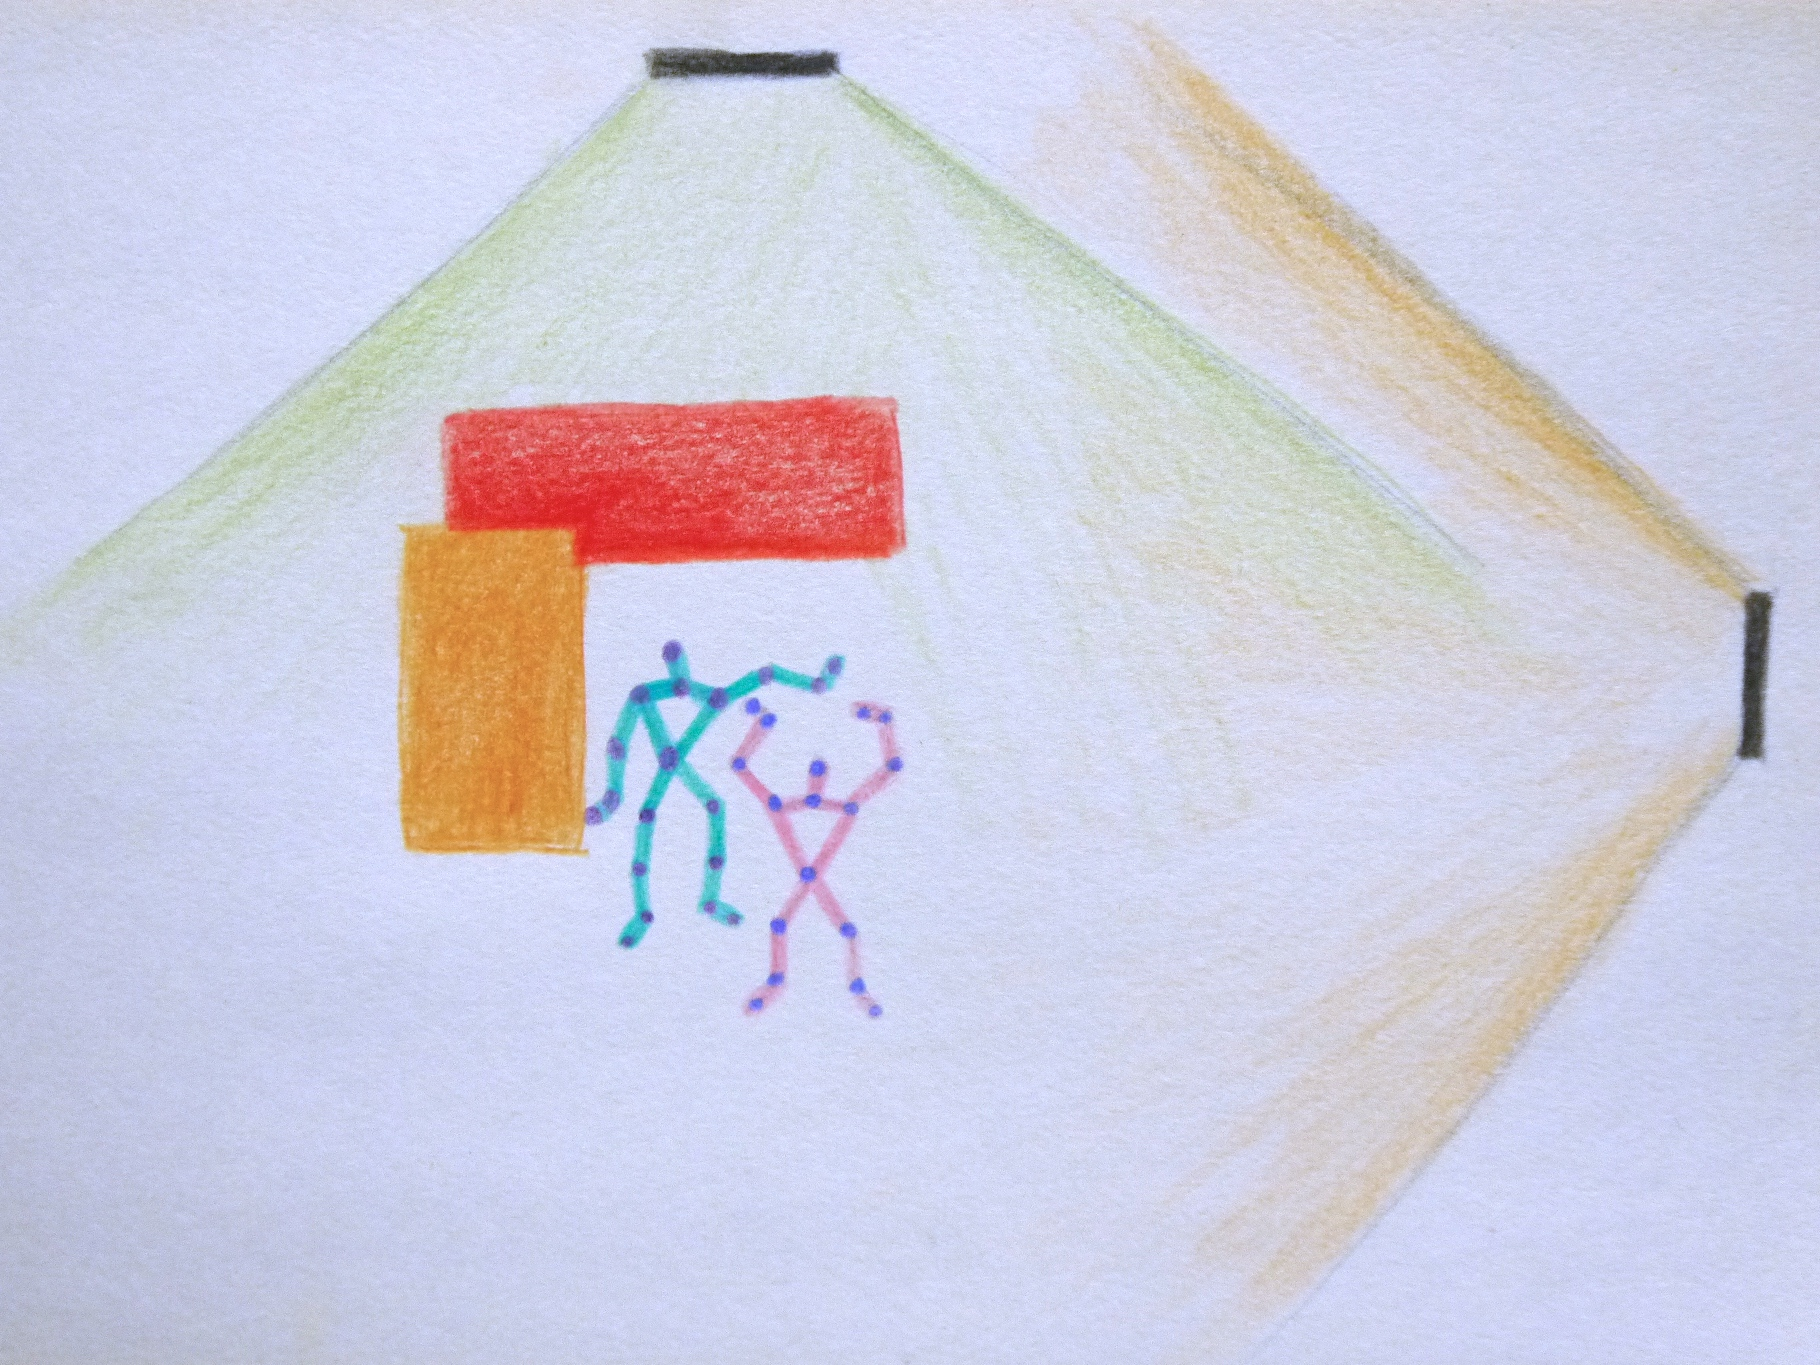
\includegraphics[width=0.8\textwidth]{occlusion}
    \caption{The problem of occlusion}
    \label{fig:occlusion_problem}
\end{figure}

\subsection{Kinect}

Kinect is a low-cost sensor for motion capturing and tracking. The sensor provides infrared, RGB, and depth streams at high frame rates.

\section{Related Work}

Tracking moving targets is challenging. Because... The section will review the state of the art techniques in people tracking.

\subsection{RGB-D}





\subsubsection{Color normalization}



\subsubsection{Feature-based tracking}

Gavrila et al extract depth features from images and match them against a hierarchy of templates to detect pedestrians in realtime [0]. Mikolajczyk1 et al detect the human body as a collection of local feature leared from training examples using Adaptive Boosting, a machine learning technique that gradually improves the model based on the errors of the previous models [3]. Lowe presents the scale-invariant feature transform (SIFT) technique to extract highly distinctive interest points from images that can be used to identify objects from different views [6].

\subsubsection{Color Histogram}
In addition to feature detection, histogram based detection techniques are also used frequently. A color histogram based people tracking system is able to keep track of moving people after occlusion and changing illumination [4].  

\subsubsection{HOG: Histogram of Oriented Gradients}

Moreover, Dalal and Bill Triggs show experimentally that Histograms of Oriented Gradient (HOG) descriptors outperform existing human detectors [1]. HOG is one of the most widely used techniques for people detection [7, 8], and subsequent work show that it can not only reliably track similar targets but also increase the performance of tracking algorithm [2, 9, 10].

The method evalutes local histogram of image gradient orientations. An image gradient is a directional change in the color intensity in a fixed-size detection window. Each dection window is divided into cells. A histogram of gradient directions is created for the the pixels within the cell. Local features can be characterized by the distribution of the local gradients. The local histograms of a group of cells, or a block, are normalized. That is, differences among the local histograms of a block are small. The normalization procedure ensures the histograms are invariant to changes in illumination and contrast. HOG is represented as a collection of normalized descriptor blocks, each describing the local features of a region in an image. The descriptor is then used to train a linear Support Vector Machine(SVM) to do person and non-person classification. To detect multiple people, the detection window is scrolled over the image at different scales and the corresponding descriptors are computed to train the SVM.

\subsubsection{HOD: Histogram of Oriented Depths}

Inspired by HOG, Spinello and Arras develop a person detector called Histogram of Oriented Depths (HOD) for dense depth data [5]. Similarly to HOG, HOD divides a fixed-size detection window into cells. Instead of encoding changes in color intensity, it computes the local oriented depth gradients and creates a histogram for each cell. The histograms of a block, or four cells, are normalized. HOG captures local 2D shape, whereas HOD captures local 3D shape. The descriptors are also taken for training a linear SVM. HOD uses the depth information to make an informed scale-space search, as opposed to the uninformed search in the HOG approach.

\subsubsection{Combo-HOD: RGB-D people detector}

Spinello and Arras propose a novel person detector that probablistically combines HOG and HOD [5]. HOG uses image data which are rich in color and texture but poor under changing illumination, and HOD uses depth data which are invariant to illumniation changes. Combo-HOD trains a HOG detector on image data and a HOD detector on depth data. The method relies on the informed scale-space search which uses HOD descriptors and HOG descriptors on the same detection window at scales that are compatible with the presence of people in the image. [Need to read the papers again]

The Kinect depth information becomes highly unreliable over eight meters from the sensor; however, using a combined approach of HOG and HOD can increase the reliability of the overall tracking algorithm. The method does not rely background segmentation nor a ground plane assumption, but it relies on heavy GPU implementation. [Discuss more results]

\subsubsection{Depth-based human model}


\subsubsection{Tracking within groups}

Munaro et al propose a depth-based sub-clustering method for detecting and tracking people within groups [10]. The method can detect people with dynamic occlusion, such as when people are standing very close or walking past each other. The tracking algorithm performs the detection and tracking association using motion, appearance, and detection confidence. An online learned classifier is also used to track people by learning negative examples from the detection process.

The proposed method consists of a voxel grid filtering procedure which reduces the size of the RGB-D point cloud for processing. It divides the depth space into voxels, where each voxel contains sample depth values that are some distance apart. A height map is obtained for each cluster using depth information, and sub-clusters are created by finding the local maxima within the height map. A bounding box is made for each cluster, where its boundary should contain a person's whole body. Then, the method applies a HOG detector to the bounding box of each sub-cluster.

For every tracked sub-cluster, a RGB color histogram is computed. The appearce of each tracked target is learned via an online classifier

The tracking module formulates the detection and tracking association

The algorithm runs at 26 frames per second and does not involve a GPU implementation.

\subsection{More papers}

Robust Tracking-by-Detection using a Detector Confidence Particle Filter

Detecting and Tracking People using an RGB-D Camera via Multiple Detector
Fusion

Real-Time Multi-Person Tracking with Detector Assisted Structure Propagation

Human Detection Using Depth Information by Kinect

3D flow estimation for human action recognition from colored point clouds

\subsection{Multiple Kinects}

\subsubsection{Calibration}

\subsubsection{Merging the FOVs}

\subsubsection{Scheduling}

Intelligent sensor-scheduling for multi-kinect-tracking

\section{Current Approach}

\section{References}

[0] Vision-Based Pedestrian Detection: The PROTECTOR System
[1] Histograms of Oriented Gradients for Human Detection
[2] Exploring Context Information for Inter-Camera Multiple Target Tracking
[3] Human Detection Based on a Probabilistic Assembly of Robust Part Detectors
[4] A COLOR HISTOGRAM BASED PEOPLE TRACKING SYSTEM
[5] People Detection in RGB-D Data
[6] Distinctive Image Features from Scale-Invariant Keypoints


[7] Pedestrian detection: A benchmark
[8] Monocular pedestrian detection: Survey and experiments
[9] People tracking in RGB-D data with on-line boosted target models
[10] Tracking people within groups with RGB-D data

\end{document}